\section{Multiresolution Analysis (MRA)}

\subsection{Orthogonal MRA}
Skalierungsfunktion (Mother scaling function $\varphi(t)$; nicht zu verwechseln mit Wavelets!): 
\[
	\varphi_{m,n}(t)=2^{-m/2} \cdot \varphi(2^{-m}\cdot t - n) = \frac{1}{\sqrt{2^{m}}} \cdot \varphi(2^{-m}\cdot t -n) = 2^{-m/2} \cdot \varphi(2^{-m}\cdot (t - 2^{m}\cdot n))
\]

\textbf{Axioms} (Anforderungen) die eine Skalierungsfunktion erfüllen muss:
\begin{enumerate}
	\item orthonormality: $ \langle \varphi_{0,n}|\varphi_{0,n'} \rangle = \delta_{n,n'} =  \begin{cases} 1 \quad n=n'\\ 0 \quad sonst  \end{cases}  $
	\item 2-scaling: $ \varphi(t) = \sqrt{2} \sum_{k \in \mathbb{Z}} h_k \cdot \varphi(2t-k) = \sum_{k \in \mathbb{Z}} h_k \cdot \varphi_{-1,k}(t) \qquad \varphi_{m,n}=\sum_{k \in \mathbb{Z}} h_k \cdot \varphi_{m-1,2n+k} $
	\item mean one: $ \varphi \text{ muss integrierbar sein und } \int_{-\infty}^{\infty}\varphi(t) \mathrm{d}t = 1 $
\end{enumerate}

(Aussage von 2-scaling: Eine Funktion wird um den Faktor 2 (in der Zeit) gestaucht. Durch verschieben, strecken bzw. stauchen (der Amplitude) und aufaddieren dieser skalierten Funktion, kann die  Ausgangsfunktion wieder dargestellt werden.)

Daraus ergeben sich folgende einfachen Konsequenzen:
\[ 
	\sum_{k \in \mathbb{Z}} h_k = \sqrt{2} \qquad \qquad (\text{z.B.: } h_0 + h_1 + h_3 + h_4 + h_5 = \sqrt{2})
\]
Double-Shift -orthogonality:
\[
	\delta_{0,n} = \sum_{k \in \mathbb{Z}} h_k h_{k-2n} 
	\qquad \qquad 
	(\text{z.B.: } h_0h_2 + h_1h_3 + h_2h_4 + h3_h5 = h_0h_4+h_1h_5 = 0 )
\]

Scale space: 
\[
	V_m = \langle \varphi_{m,n}|n \in \mathbb{Z}  \rangle = \{ ...,\varphi_{m,-1},\varphi_{m,0}, \varphi_{m,1}, \varphi_{m,2},... \}
	\qquad \qquad
	V_mf = \sum_{n \in \mathbb{Z}} u_{m,n}\varphi_{m,n} \quad \text{mit } u_{m,n}=\langle \varphi_{m,n}|f \rangle
\]

Lokalisation:
\[  
	m \rightarrow -\infty \quad ||f-V_mf||^2 \rightarrow 0 \quad (\text{finer (feiner)})
	\qquad \qquad
	m \rightarrow +\infty \quad ||V_mf||^2 \rightarrow 0 \quad (\text{coarser (gröber)})
\]

Detail space (Detailinformation):
\[
	W_m = \langle \psi_{m,n} | n \in \mathbb{Z} \rangle = \{ ...,\psi_{m,-1},\psi_{m,0}, \psi_{m,1}, \psi_{m,2},... \}
	\qquad \qquad
	W_mf = \sum_{n \in \mathbb{Z}} \nu_{m,n}\psi_{m,n} \quad \text{mit } \nu_{m,n}=\langle \psi_{m,n}|f \rangle
\]
Räume (je weiter nach rechts (je kleiner m), desto grösser der Raum):
\[ V_{m-1} = V_m \oplus W_m  \qquad \qquad ...\subset V_{m+1} \subset V_{m} \subset V_{m-1} \subset ... \]

Wavelet:
\[
	\psi_{m,n} = \sum_{k \in \mathbb{Z}} g_k \varphi_{m-1,2n+k} 
	\qquad \qquad 
	\left(\psi_{0,0}=\sum_{k \in \mathbb{Z}} (-1)^k h_{l-k} \sqrt{2}  \varphi_{0,0}(2t-k) = \sum_{k \in \mathbb{Z}} g_k \varphi_{-1,k} \quad \underbrace{l \in \mathbb{Z}_{ungerade}}_{\text{frei wählbar}} \right)
\]

\textbf{Fast Wavelet Transform} (Decomposition / Reconstruction):
\[
	\boxed{\begin{array}{ccccc}
		u_m & \xrightarrow{A} & u_{m+1} & \xrightarrow{A} & u_{m+2} \\
		& \searrow^{D} & & \searrow^{D} & \\
		& & \nu_{m+1} & & \nu_{m+2} \\
	\end{array}}
	\qquad \qquad \qquad \qquad
	\boxed{\begin{array}{ccccc}
		u_{m+2} & \xrightarrow{\tilde{A}} & u_{m+1} & \xrightarrow{\tilde{A}} & u_{m} \\
		& \nearrow_{\tilde{D}} & & \nearrow_{\tilde{D}} & \\
		\nu_{m+2}& & \nu_{m+1} & & \\
	\end{array}}
\]

\[  
	u_{m+1,n} = \sum_{k \in  \mathbb{Z}} h_{k-2n} u_{m,k} \quad \nu_{m+1,n} = \sum_{k \in  \mathbb{Z}} g_{k-2n} u_{m,k}
	\qquad \qquad
	u_{m,n} = \sum_{k \in  \mathbb{Z}} h_{n-2k} u_{m+1,k} + g_{n-2k} \nu_{m+1,k}
\]

\[
	A(x)_n = \sum_{k \in  \mathbb{Z}} h_{k-2n} x_k
	\qquad \qquad \qquad \qquad
	\tilde{A}(x)_n = \sum_{k \in  \mathbb{Z}} h_{n-2k} x_k
\]

\[
	D(x)_n = \sum_{k \in  \mathbb{Z}} g_{k-2n} x_k
	\qquad \qquad \qquad \qquad
	\tilde{D}(x)_n = \sum_{k \in  \mathbb{Z}} g_{n-2k} x_k
\]


Vereinfachung des Analyseschritts für die Handrechnung $k-2n=l\rightarrow k=l+2n$:
\[ 
	u_{m+1,n} = \sum_{l} h_{l} u_{m,l+2n}
	\qquad \qquad \qquad \qquad
	\nu_{m+1,n} = \sum_{l} g_{l} u_{m,l+2n}
\]


\subsection{Biorthogonal MRA}

\textbf{Axioms} (Anforderungen) die eine Skalierungsfunktion erfüllen muss:
\begin{enumerate}
	\item biorthogonality: $ \langle \varphi_{m,n}|\tilde{\varphi}_{p,q} \rangle = \delta_{m,p}\cdot \delta_{n,p} \qquad \qquad \left( \langle \varphi_{0,n}|\tilde{\varphi}_{0,0} \rangle = \delta_{0,n} \right)$
	\item 2-scaling: $ \varphi_{0,0}(t) = \sum_{k \in \mathbb{Z}} h_k \cdot \varphi_{-1,k}(t) \qquad \qquad  \tilde{\varphi}_{0,0}(t) = \sum_{k \in \mathbb{Z}} h_k \cdot \tilde{\varphi}_{-1,k}(t) $
	\item mean one: $ \int_{-\infty}^{\infty}\varphi(t) \mathrm{d}t = 1 \qquad \qquad \int_{-\infty}^{\infty}\tilde{\varphi}(t) \mathrm{d}t = 1$
\end{enumerate}

Einfache Konsequenzen sind:
\[ 
	\sum_{k \in  \mathbb{Z}} h_k = \sum_{k \in  \mathbb{Z}} \tilde{h}_k = \sqrt{2} 
	\qquad \qquad
	\text{Double shift orthogonality:} \quad \sum_{k \in  \mathbb{Z}} h_k \tilde{h}_{k+2n} = \delta_{0,n}
\]

$  
	\text{Analyse-Funktion: } \varphi_{m,n} \quad \psi_{m,n}
	\qquad \qquad
	\text{Synthese-Funktion: } \tilde{\varphi}_{m,n} \quad \tilde{\psi}_{m,n}
$

\vspace{2mm}

Wavelet:
\[
	\psi_{0,0}=\sum_{k \in \mathbb{Z}} (-1)^k \tilde{h}_{l-k} \sqrt{2}  \varphi_{0,0}(2t-k) = \sum_{k \in \mathbb{Z}} g_k \varphi_{-1,k} 
	\qquad
	\tilde{\psi}_{0,0}=\sum_{k \in \mathbb{Z}} (-1)^k h_{l-k} \sqrt{2}  \tilde{\psi}_{0,0}(2t-k) = \sum_{k \in \mathbb{Z}} \tilde{g}_k \tilde{\psi}_{-1,k} 
	\qquad 
	\underbrace{l \in \mathbb{Z}_{odd}}_{\text{frei wählbar}}
\]


\subsection{Filterbank Beschreibung}
Up-/ Downsampling: $ S(z) (\downarrow 2)(\uparrow 2) = \frac{1}{2} (S(z)+S(-z) $

\vspace{-2cm}

\begin{flushright}
	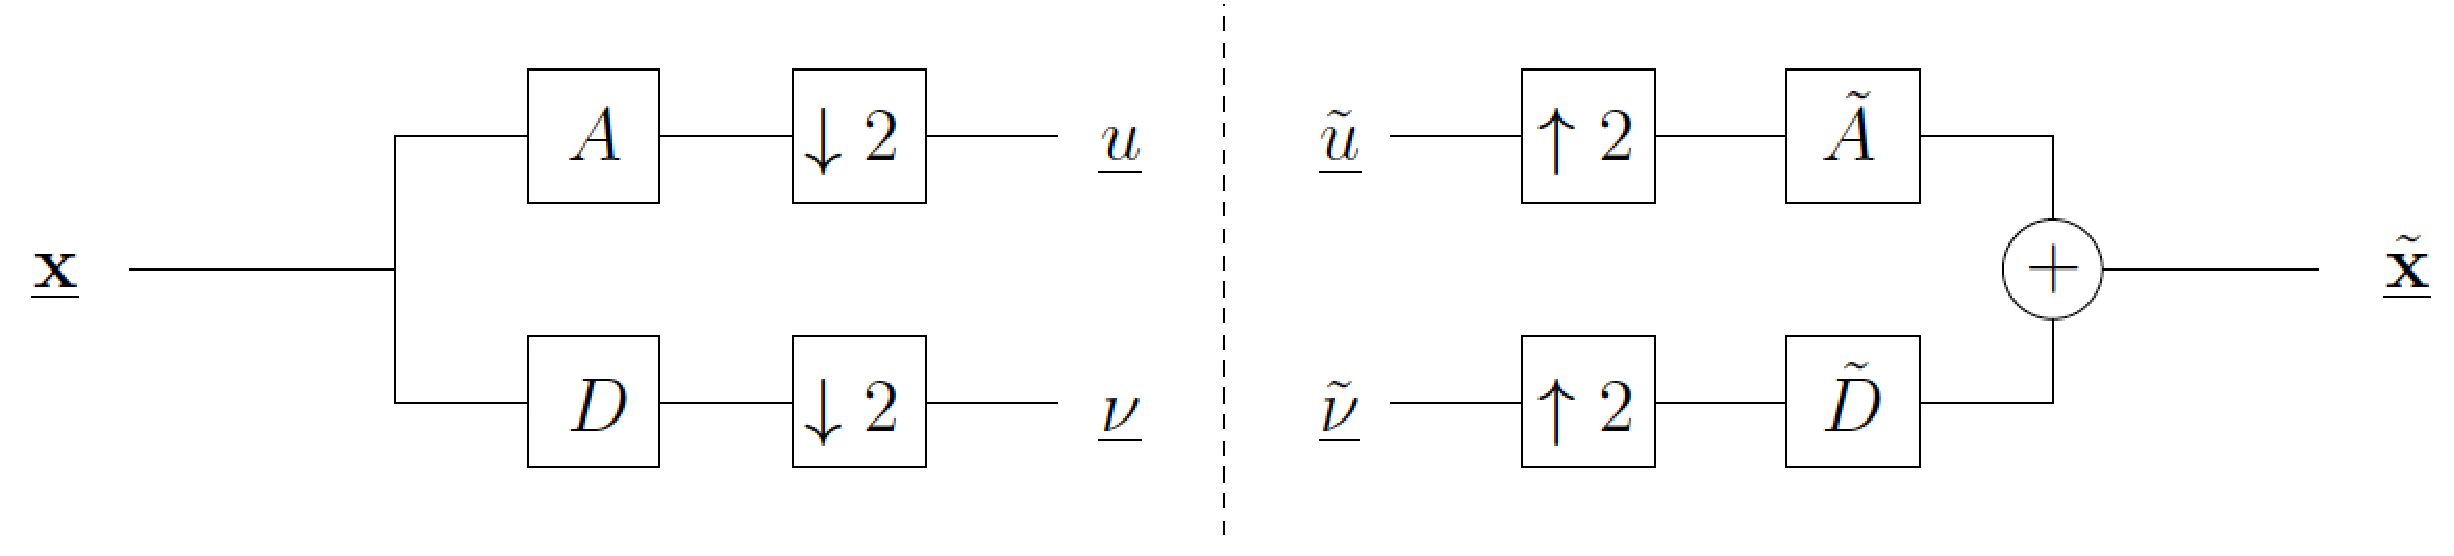
\includegraphics[width=0.5\textwidth]{content/FilterBank.pdf} 
\end{flushright}
 
\vspace{-0.5cm}

Filterbank (durch $-(-1)^k$ werden alle geraden Koeffizienten gelöscht ($=0$) ):
\[  
	\underbrace{\tilde{A}(z) A(z)}_{M(z)} + \underbrace{\tilde{D}(z)D(z)}_{-(-1)^k M(-z)} = M(z)-(-1)^kM(-z) = 2
	\qquad \qquad
	\tilde{A}(z)A(-z) + \tilde{D}(z)D(-z) = 0
\]

\subsubsection{Orthogonale Filterkoeffizienten}
Zusammenhang der Filter (shift: $(-z)^k$, inverse Reihenfolge durch $z^{-1}$, alternierendes Vorzeichen$(\pm)$ durch einsetzen von $-z$):
%TODO wo ist z^0 und wo z^n (Skript seite 27 + application db2 vergleichen???)
\[  
	\tilde{A}(z) = A(z^{-1})
	\qquad \qquad
	D(z) = \tilde{D}(z^{-1}) = (-z)^l\tilde{A}(-z) \qquad l\text{: ungerade, frei wählbar}
\]
\[  
	A = [h_0,...,h_n] \qquad
	\tilde{A} = [h_n,...,h_0]
	\qquad \qquad
	D = [h_n,-h_{n-1}, h_{n-2},...,h_1,-h_0] \qquad
	\tilde{D} = [-h_0,h_1, -h_2,...,-h_{n-1},h_n]
\]

Mit einer orthogonalen Filterbank hat man Quadrature Mirror Filter Eigenschaften:\\
 $|\hat{h}(\xi)|^2 + |\hat{g}(\xi)|^2 = |\hat{\tilde{h}}(\xi)|^2 + |\hat{\tilde{g}}(\xi)|^2 = 2$

\subsubsection{Biorthogonal Filterkoeffizienten}

Zusammenhang der Filter (shift: $(-z)^k$ bzw. $-z^{-k}$, alternierendes Vorzeichen$(\pm)$ durch einsetzen von $-z$):
%TODO wo ist z^0 und wo z^n (Skript seite 27 + application db2 vergleichen???)
\[ 
	D(z) = (-z)^{-l}\tilde{A}(-z^{-1}) \qquad \qquad \tilde{D}(z) = (-z)^{l}A(-z^{-1})  \qquad l\text{: ungerade, frei wählbar}
\]

